\section{The Axiom of Choice}
        \begin{fdefinition}{Functions}{Function}
            A function from a set $A$ to a set $B$ is a subset
            $f\subseteq{A}\times{B}$, denoted $f:A\rightarrow{B}$, such that
            for all $x\in{A}$ there is a unique $y\in{B}$ such that
            $(x,y)\in{f}$. The set $A$ is called the domain of $f$, and the
            set $B$ is called the codomain.
        \end{fdefinition}
        We're used to hearing that a function is a rule that assigns to an
        input value $x$ some output value $f(x)$. It may seem hard to justify,
        then, why we've defined a function as a subset of the Cartesian
        product. But note the requirement that, for each $x\in{A}$, there is a
        \textit{unique} $y\in{B}$ such that $(x,y)\in{f}$. We call this unique
        element the \textit{image} of $x$ under the function $f$ and write
        $y=f(x)$. The condition that there is a unique such value $y$ to each
        $x$ is called the \textit{vertical line test} when graphing functions
        of the form $f:\mathbb{R}\rightarrow\mathbb{R}$
        (Fig.~\ref{fig:Function_R_to_R_Subset_Cart_Prod}). Simply, given such
        a function, if one draws a vertical line in the plane, then it must
        intersect the graph of $f$ once and only once. This provides a
        quick means of discerning functions from non-functions.
        \par\hfill\par
        Any curve that we draw left-to-right, without picking up the pencil,
        will be a valid function
        (See Fig.~\ref{fig:Function_R_to_R_Subset_Cart_Prod}).
        \begin{figure}[H]
            \centering
            %--------------------------------Dependencies----------------------------------%
%   xcolor                                                                     %
%   amssymb                                                                    %
%   tikz                                                                       %
%       arrows.meta                                                            %
%-------------------------------Main Document----------------------------------%
\begin{tikzpicture}[%
    >=Latex,
    line width=0.2mm,
    line cap=round,
    scale=1.2
]
    % Coorindates for the curve.
    \coordinate (P1) at (-4.00, -2.00);
    \coordinate (P2) at (-2.00, -3.00);
    \coordinate (P3) at ( 0.00,  0.00);
    \coordinate (P4) at ( 2.00,  3.00);
    \coordinate (P5) at ( 4.00,  3.90);

    % Draw a green mesh indicating the Cartesian plane.
    \foreach\x in {-40, -39, ..., 39}{
        \draw[draw=green, line width=0.1mm] (\x/10, -4) to (-4, \x/10);
        \draw[draw=green, line width=0.1mm] (4, \x/10)  to (\x/10, 4);
    }
    \draw[draw=green, line width=0.1mm] (4, 4)  to (4, 4);

    \begin{scope}[thick, font=\Large]
        \draw[<->] (-4.3,  0.0) to (4.3, 0.0) node [above] {$\mathbb{R}$};
        \draw[<->] ( 0.0, -4.3) to (0.0, 4.3) node [right] {$\mathbb{R}$};
    \end{scope}

    \draw[draw=blue] (P1) to [out=-30, in=150]  (P2)
                          to [out=-30, in=210]  (P3)
                          to [out=30,  in=180]  (P4)
                          to [out=0,   in=200]  (P5);
    \draw[fill=white, draw=white] 
        (1.3, 2.0) rectangle node {$\textcolor{blue}{f}$} (1.6, 1.4);
\end{tikzpicture}
            \caption[Example of a Function
                     $f:\mathbb{R}\rightarrow\mathbb{R}$]
                    {Example of a function
                     $f:\mathbb{R}\rightarrow\mathbb{R}$.
                     The Cartesian product $\mathbb{R}\times\mathbb{R}$ is
                     shown in \textcolor{green!80!black}{green}, and the
                     function $f\subseteq\mathbb{R}\times\mathbb{R}$ is shown
                     in \textcolor{blue}{blue}.}
            \label{fig:Function_R_to_R_Subset_Cart_Prod}
        \end{figure}
        \begin{lexample}{}{SQRT_is_Not_a_Function}
            Let $g\subseteq\mathbb{R}\times\mathbb{R}$ be defined as follows:
            \begin{equation}
                g=\big\{\;(x,y)\in\mathbb{R}^{2}\,:\,y^{2}=x\;\big\}
            \end{equation}
            It is tempting to label $g$ by writing $g(x)=\sqrt{x}$, but $g$ is
            not a function for it fails two of the requirements of a function.
            Firstly, for any $x>0$, there are two values $y_{1}$ and $y_{2}$
            whose square is equal to $x$. Indeed, if $y_{1}$ is one such value,
            then setting $y_{2}=\minus{y}_{1}$ will result in a second
            distinct value. Thus $g$ does not have the uniqueness property
            required for functions. Moreover, if $x<0$, then there is no such
            value $y\in\mathbb{R}$ such that $(x,y)\in{g}$, and thus $g$ also
            lacks the existence property. In terms of the vertical line test,
            there are points $x$ such that the vertical line through
            $(x,\,0)$ intersects $g$ twice, and there are points such that the
            vertical line does not intersect at all. The graph of $g$ is shown
            in Fig.~\ref{fig:SQRT_Not_a_Function}.
        \end{lexample}
        We need not only consider functions of the for
        $f:\mathbb{R}\rightarrow\mathbb{R}$, nor functions
        $f:\mathcal{U}\rightarrow\mathcal{V}$, where $\mathcal{U}$ and
        $\mathcal{V}$ are subsets of $\mathbb{R}$, and we can allow for
        arbitrary abstract functions.
        \begin{figure}[H]
            \centering
            %--------------------------------Dependencies----------------------------------%
%   xcolor                                                                     %
%   amssymb                                                                    %
%   tikz                                                                       %
%       arrows.meta                                                            %
%       patterns                                                               %
%-------------------------------Main Document----------------------------------%
\begin{tikzpicture}[%
    >=Latex,
    line width=0.2mm,
    line cap=round,
    scale=1.2
]
    % Coorindates for the curve.
    \coordinate (P1) at (-3.85, -2.00);
    \coordinate (P2) at (-2.00, -3.00);
    \coordinate (P3) at ( 0.00,  0.00);
    \coordinate (P4) at ( 2.00,  3.00);
    \coordinate (P5) at ( 3.85,  3.80);

    \draw[%
        pattern=north west lines,
        pattern color=Green!80!Black,
        opacity=0.5,
        draw=white
    ]   (-3.9, -3.9) rectangle (3.9, 3.9);

    \begin{scope}[thick, font=\Large]
        \draw[<->] (-4.2, 0) to (4.2, 0) node [above] {$\mathbb{R}$};
        \draw[<->] (0, -4.2) to (0, 4.2) node [right] {$\mathbb{R}$};
    \end{scope}

    \draw[draw=red] (3.880000, -1.969772) to (3.840000, -1.959592)
                                          to (3.800000, -1.949359)
                                          to (3.760000, -1.939072)
                                          to (3.720000, -1.928730)
                                          to (3.680000, -1.918333)
                                          to (3.640000, -1.907878)
                                          to (3.600000, -1.897367)
                                          to (3.560000, -1.886796)
                                          to (3.520000, -1.876166)
                                          to (3.480000, -1.865476)
                                          to (3.440000, -1.854724)
                                          to (3.400000, -1.843909)
                                          to (3.360000, -1.833030)
                                          to (3.320000, -1.822087)
                                          to (3.280000, -1.811077)
                                          to (3.240000, -1.800000)
                                          to (3.200000, -1.788854)
                                          to (3.160000, -1.777639)
                                          to (3.120000, -1.766352)
                                          to (3.080000, -1.754993)
                                          to (3.040000, -1.743560)
                                          to (3.000000, -1.732051)
                                          to (2.960000, -1.720465)
                                          to (2.920000, -1.708801)
                                          to (2.880000, -1.697056)
                                          to (2.840000, -1.685230)
                                          to (2.800000, -1.673320)
                                          to (2.760000, -1.661325)
                                          to (2.720000, -1.649242)
                                          to (2.680000, -1.637071)
                                          to (2.640000, -1.624808)
                                          to (2.600000, -1.612452)
                                          to (2.560000, -1.600000)
                                          to (2.520000, -1.587451)
                                          to (2.480000, -1.574802)
                                          to (2.440000, -1.562050)
                                          to (2.400000, -1.549193)
                                          to (2.360000, -1.536229)
                                          to (2.320000, -1.523155)
                                          to (2.280000, -1.509967)
                                          to (2.240000, -1.496663)
                                          to (2.200000, -1.483240)
                                          to (2.160000, -1.469694)
                                          to (2.120000, -1.456022)
                                          to (2.080000, -1.442221)
                                          to (2.040000, -1.428286)
                                          to (2.000000, -1.414214)
                                          to (1.960000, -1.400000)
                                          to (1.920000, -1.385641)
                                          to (1.880000, -1.371131)
                                          to (1.840000, -1.356466)
                                          to (1.800000, -1.341641)
                                          to (1.760000, -1.326650)
                                          to (1.720000, -1.311488)
                                          to (1.680000, -1.296148)
                                          to (1.640000, -1.280625)
                                          to (1.600000, -1.264911)
                                          to (1.560000, -1.249000)
                                          to (1.520000, -1.232883)
                                          to (1.480000, -1.216553)
                                          to (1.440000, -1.200000)
                                          to (1.400000, -1.183216)
                                          to (1.360000, -1.166190)
                                          to (1.320000, -1.148913)
                                          to (1.280000, -1.131371)
                                          to (1.240000, -1.113553)
                                          to (1.200000, -1.095445)
                                          to (1.160000, -1.077033)
                                          to (1.120000, -1.058301)
                                          to (1.080000, -1.039230)
                                          to (1.040000, -1.019804)
                                          to (1.000000, -1.000000)
                                          to (0.960000, -0.979796)
                                          to (0.920000, -0.959166)
                                          to (0.880000, -0.938083)
                                          to (0.840000, -0.916515)
                                          to (0.800000, -0.894427)
                                          to (0.760000, -0.871780)
                                          to (0.720000, -0.848528)
                                          to (0.680000, -0.824621)
                                          to (0.640000, -0.800000)
                                          to (0.600000, -0.774597)
                                          to (0.560000, -0.748331)
                                          to (0.520000, -0.721110)
                                          to (0.480000, -0.692820)
                                          to (0.440000, -0.663325)
                                          to (0.400000, -0.632456)
                                          to (0.360000, -0.600000)
                                          to (0.320000, -0.565685)
                                          to (0.280000, -0.529150)
                                          to (0.240000, -0.489898)
                                          to (0.200000, -0.447214)
                                          to (0.160000, -0.400000)
                                          to (0.120000, -0.346410)
                                          to (0.080000, -0.282843)
                                          to (0.040000, -0.200000)
                                          to (0.000000, 0.000000) 
                                          to (0.040000, 0.200000)
                                          to (0.080000, 0.282843)
                                          to (0.120000, 0.346410)
                                          to (0.160000, 0.400000)
                                          to (0.200000, 0.447214)
                                          to (0.240000, 0.489898)
                                          to (0.280000, 0.529150)
                                          to (0.320000, 0.565685)
                                          to (0.360000, 0.600000)
                                          to (0.400000, 0.632456)
                                          to (0.440000, 0.663325)
                                          to (0.480000, 0.692820)
                                          to (0.520000, 0.721110)
                                          to (0.560000, 0.748331)
                                          to (0.600000, 0.774597)
                                          to (0.640000, 0.800000)
                                          to (0.680000, 0.824621)
                                          to (0.720000, 0.848528)
                                          to (0.760000, 0.871780)
                                          to (0.800000, 0.894427)
                                          to (0.840000, 0.916515)
                                          to (0.880000, 0.938083)
                                          to (0.920000, 0.959166)
                                          to (0.960000, 0.979796)
                                          to (1.000000, 1.000000)
                                          to (1.040000, 1.019804)
                                          to (1.080000, 1.039230)
                                          to (1.120000, 1.058301)
                                          to (1.160000, 1.077033)
                                          to (1.200000, 1.095445)
                                          to (1.240000, 1.113553)
                                          to (1.280000, 1.131371)
                                          to (1.320000, 1.148913)
                                          to (1.360000, 1.166190)
                                          to (1.400000, 1.183216)
                                          to (1.440000, 1.200000)
                                          to (1.480000, 1.216553)
                                          to (1.520000, 1.232883)
                                          to (1.560000, 1.249000)
                                          to (1.600000, 1.264911)
                                          to (1.640000, 1.280625)
                                          to (1.680000, 1.296148)
                                          to (1.720000, 1.311488)
                                          to (1.760000, 1.326650)
                                          to (1.800000, 1.341641)
                                          to (1.840000, 1.356466)
                                          to (1.880000, 1.371131)
                                          to (1.920000, 1.385641)
                                          to (1.960000, 1.400000)
                                          to (2.000000, 1.414214)
                                          to (2.040000, 1.428286)
                                          to (2.080000, 1.442221)
                                          to (2.120000, 1.456022)
                                          to (2.160000, 1.469694)
                                          to (2.200000, 1.483240)
                                          to (2.240000, 1.496663)
                                          to (2.280000, 1.509967)
                                          to (2.320000, 1.523155)
                                          to (2.360000, 1.536229)
                                          to (2.400000, 1.549193)
                                          to (2.440000, 1.562050)
                                          to (2.480000, 1.574802)
                                          to (2.520000, 1.587451)
                                          to (2.560000, 1.600000)
                                          to (2.600000, 1.612452)
                                          to (2.640000, 1.624808)
                                          to (2.680000, 1.637071)
                                          to (2.720000, 1.649242)
                                          to (2.760000, 1.661325)
                                          to (2.800000, 1.673320)
                                          to (2.840000, 1.685230)
                                          to (2.880000, 1.697056)
                                          to (2.920000, 1.708801)
                                          to (2.960000, 1.720465)
                                          to (3.000000, 1.732051)
                                          to (3.040000, 1.743560)
                                          to (3.080000, 1.754993)
                                          to (3.120000, 1.766352)
                                          to (3.160000, 1.777639)
                                          to (3.200000, 1.788854)
                                          to (3.240000, 1.800000)
                                          to (3.280000, 1.811077)
                                          to (3.320000, 1.822087)
                                          to (3.360000, 1.833030)
                                          to (3.400000, 1.843909)
                                          to (3.440000, 1.854724)
                                          to (3.480000, 1.865476)
                                          to (3.520000, 1.876166)
                                          to (3.560000, 1.886796)
                                          to (3.600000, 1.897367)
                                          to (3.640000, 1.907878)
                                          to (3.680000, 1.918333)
                                          to (3.720000, 1.928730)
                                          to (3.760000, 1.939072)
                                          to (3.800000, 1.949359)
                                          to (3.840000, 1.959592)
                                          to (3.880000, 1.969772);
    \draw[fill=white, draw=white] 
        (1.3, 2.0) rectangle node {$\textcolor{red}{g}$} (1.6, 1.5);
\end{tikzpicture}
            \caption[Example of a Non-Function]
                {$g\subseteq\mathbb{R}\times\mathbb{R}$ is not a function
                 since it fails the vertical line test.}
            \label{fig:SQRT_Not_a_Function}
        \end{figure}
        \begin{lexample}{Abstract Functions}{Abstract_Functions}
            Let $A$ and $B$ be sets defined as follows:
            \par
            \begin{subequations}
                \begin{minipage}[b]{0.49\textwidth}
                    \centering
                    \begin{equation}
                        A=\{\,1,\,2,\,3,\,4\,\}
                    \end{equation}
                \end{minipage}
                \hfill
                \begin{minipage}[b]{0.49\textwidth}
                    \centering
                    \begin{equation}
                        B=\{\,a,\,b,\,c\,\}
                    \end{equation}
                \end{minipage}
            \end{subequations}
            \par\vspace{2.5ex}
            Similar to the vertical line test, we can devise a visual to
            discerning functions from non-functions for abstract sets.
            We represents the elements of $A$ and $B$ as points in some blob
            in the plane, and then draw arrows between the points
            $x\in{A}$ and $y\in{b}$ indicating that $(x,\,y)\in{f}$.
            This allows us to discern between functions and non-functions.
            Every point in $A$ must be mapped to a unique point in $B$.
            That is, every point in $A$ must have one and only one arrow
            connecting it to some point in $B$. Examples of valid functions
            are shown in Fig.~\ref{fig:Abstract_Functions}, and non-functions
            are shown in Fig.~\ref{fig:Abstract_Non_Functions}.
        \end{lexample}
        \begin{figure}[H]
            \centering
            \begin{subfigure}[b]{0.49\textwidth}
                \centering
                \resizebox{\textwidth}{!}{%
                    %--------------------------------Dependencies----------------------------------%
%   tikz                                                                       %
%       arrows.meta                                                            %
%-------------------------------Main Document----------------------------------%
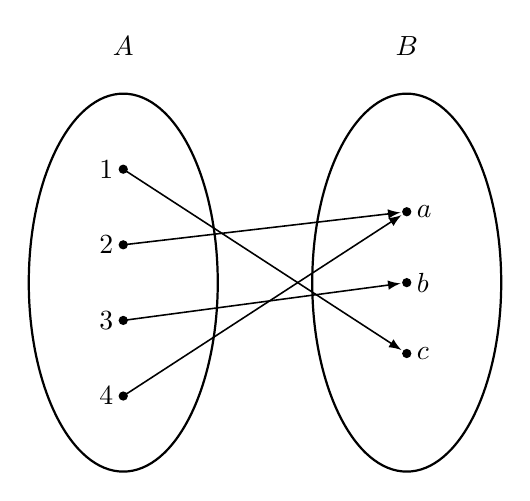
\begin{tikzpicture}[%
    >=latex,
    line width=0.2mm,
    line cap=round,
    scale=1.2
]
    % Coorindates.
    \coordinate (a) at ( 1.5,  0.75);
    \coordinate (b) at ( 1.5, -0.00);
    \coordinate (c) at ( 1.5, -0.75);
    \coordinate (1) at (-1.5,  1.20);
    \coordinate (2) at (-1.5,  0.40);
    \coordinate (3) at (-1.5, -0.40);
    \coordinate (4) at (-1.5, -1.20);
    \coordinate (A) at (-1.5,  2.50);
    \coordinate (B) at ( 1.5,  2.50);

    % Ellipses representing the sets A and B.
    \draw[thick] (-1.5, 0.0) ellipse (1 and 2);
    \draw[thick] ( 1.5, 0.0) ellipse (1 and 2);

    % Draw circles for the various points.
    \draw[fill=black] (a) circle (0.4mm);
    \draw[fill=black] (b) circle (0.4mm);
    \draw[fill=black] (c) circle (0.4mm);
    \draw[fill=black] (1) circle (0.4mm);
    \draw[fill=black] (2) circle (0.4mm);
    \draw[fill=black] (3) circle (0.4mm);
    \draw[fill=black] (4) circle (0.4mm);

    % Draw paths indicating mappings.
    \begin{scope}[->]
        \draw[shorten >=0.8mm] (1) to (c);
        \draw[shorten >=0.8mm] (2) to (a);
        \draw[shorten >=0.8mm] (3) to (b);
        \draw[shorten >=0.8mm] (4) to (a);
    \end{scope}

    % Labels.
    \node at (A)         {$A$};
    \node at (B)         {$B$};
    \node at (a) [right] {$a$};
    \node at (b) [right] {$b$};
    \node at (c) [right] {$c$};
    \node at (1) [left]  {$1$};
    \node at (2) [left]  {$2$};
    \node at (3) [left]  {$3$};
    \node at (4) [left]  {$4$};
\end{tikzpicture}
                }
                \subcaption{A Valid Function.}
            \end{subfigure}
            \begin{subfigure}[b]{0.49\textwidth}
                \centering
                \resizebox{\textwidth}{!}{%
                    %--------------------------------Dependencies----------------------------------%
%   tikz                                                                       %
%       arrows.meta                                                            %
%-------------------------------Main Document----------------------------------%
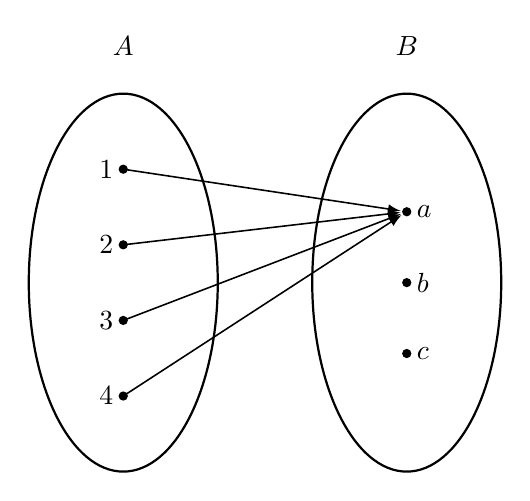
\begin{tikzpicture}[%
    >=latex,
    line width=0.2mm,
    line cap=round,
    scale=1.2
]
    % Coorindates.
    \coordinate (a) at ( 1.5,  0.75);
    \coordinate (b) at ( 1.5, -0.00);
    \coordinate (c) at ( 1.5, -0.75);
    \coordinate (1) at (-1.5,  1.20);
    \coordinate (2) at (-1.5,  0.40);
    \coordinate (3) at (-1.5, -0.40);
    \coordinate (4) at (-1.5, -1.20);
    \coordinate (A) at (-1.5,  2.50);
    \coordinate (B) at ( 1.5,  2.50);

    % Ellipses representing the sets A and B.
    \draw[thick] (-1.5, 0.0) ellipse (1 and 2);
    \draw[thick] ( 1.5, 0.0) ellipse (1 and 2);

    % Draw circles for the various points.
    \draw[fill=black] (a) circle (0.4mm);
    \draw[fill=black] (b) circle (0.4mm);
    \draw[fill=black] (c) circle (0.4mm);
    \draw[fill=black] (1) circle (0.4mm);
    \draw[fill=black] (2) circle (0.4mm);
    \draw[fill=black] (3) circle (0.4mm);
    \draw[fill=black] (4) circle (0.4mm);

    % Draw paths indicating mappings.
    \begin{scope}[->]
        \draw[shorten >=0.8mm] (1) to (a);
        \draw[shorten >=0.8mm] (2) to (a);
        \draw[shorten >=0.8mm] (3) to (a);
        \draw[shorten >=0.8mm] (4) to (a);
    \end{scope}

    % Labels.
    \node at (A)         {$A$};
    \node at (B)         {$B$};
    \node at (a) [right] {$a$};
    \node at (b) [right] {$b$};
    \node at (c) [right] {$c$};
    \node at (1) [left]  {$1$};
    \node at (2) [left]  {$2$};
    \node at (3) [left]  {$3$};
    \node at (4) [left]  {$4$};
\end{tikzpicture}
                }
                \subcaption{Another Valid Function.}
            \end{subfigure}
            \caption{Visual for Abstract Functions}
            \label{fig:Abstract_Functions}
        \end{figure}
        \begin{figure}[H]
            \centering
            \begin{subfigure}[b]{0.49\textwidth}
                \centering
                \resizebox{\textwidth}{!}{%
                    %--------------------------------Dependencies----------------------------------%
%   tikz                                                                       %
%       arrows.meta                                                            %
%-------------------------------Main Document----------------------------------%
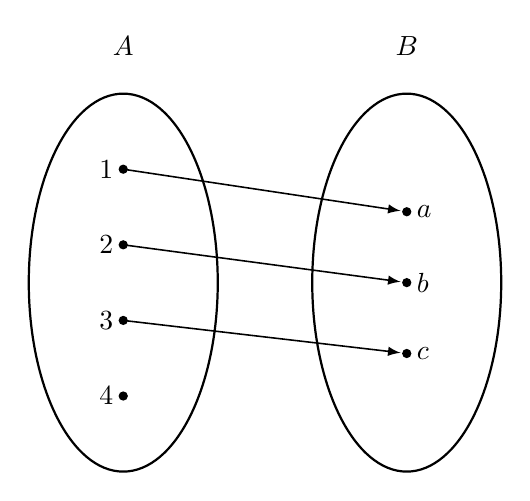
\begin{tikzpicture}[%
    >=latex,
    line width=0.2mm,
    line cap=round,
    scale=1.2
]
    % Coorindates.
    \coordinate (a) at ( 1.5,  0.75);
    \coordinate (b) at ( 1.5, -0.00);
    \coordinate (c) at ( 1.5, -0.75);
    \coordinate (1) at (-1.5,  1.20);
    \coordinate (2) at (-1.5,  0.40);
    \coordinate (3) at (-1.5, -0.40);
    \coordinate (4) at (-1.5, -1.20);
    \coordinate (A) at (-1.5,  2.50);
    \coordinate (B) at ( 1.5,  2.50);

    % Ellipses representing the sets A and B.
    \draw[thick] (-1.5, 0.0) ellipse (1 and 2);
    \draw[thick] ( 1.5, 0.0) ellipse (1 and 2);

    % Draw circles for the various points.
    \draw[fill=black] (a) circle (0.4mm);
    \draw[fill=black] (b) circle (0.4mm);
    \draw[fill=black] (c) circle (0.4mm);
    \draw[fill=black] (1) circle (0.4mm);
    \draw[fill=black] (2) circle (0.4mm);
    \draw[fill=black] (3) circle (0.4mm);
    \draw[fill=black] (4) circle (0.4mm);

    % Draw paths indicating mappings.
    \begin{scope}[->]
        \draw[shorten >=0.8mm] (1) to (a);
        \draw[shorten >=0.8mm] (2) to (b);
        \draw[shorten >=0.8mm] (3) to (c);
    \end{scope}

    % Labels.
    \node at (A)         {$A$};
    \node at (B)         {$B$};
    \node at (a) [right] {$a$};
    \node at (b) [right] {$b$};
    \node at (c) [right] {$c$};
    \node at (1) [left]  {$1$};
    \node at (2) [left]  {$2$};
    \node at (3) [left]  {$3$};
    \node at (4) [left]  {$4$};
\end{tikzpicture}
                }
                \subcaption{Fails Existence.}
            \end{subfigure}
            \begin{subfigure}[b]{0.49\textwidth}
                \centering
                \resizebox{\textwidth}{!}{%
                    %--------------------------------Dependencies----------------------------------%
%   tikz                                                                       %
%       arrows.meta                                                            %
%-------------------------------Main Document----------------------------------%
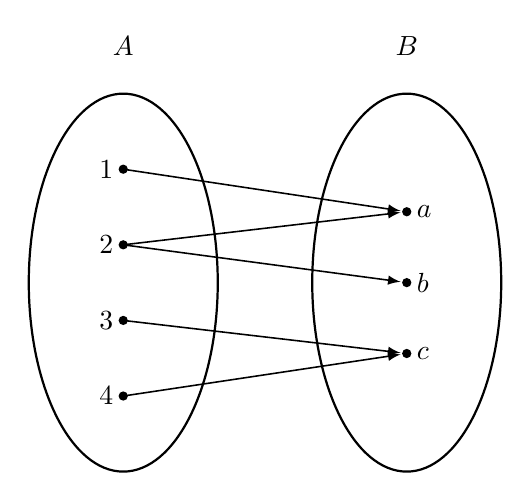
\begin{tikzpicture}[%
    >=latex,
    line width=0.2mm,
    line cap=round,
    scale=1.2
]
    % Coorindates.
    \coordinate (a) at ( 1.5,  0.75);
    \coordinate (b) at ( 1.5, -0.00);
    \coordinate (c) at ( 1.5, -0.75);
    \coordinate (1) at (-1.5,  1.20);
    \coordinate (2) at (-1.5,  0.40);
    \coordinate (3) at (-1.5, -0.40);
    \coordinate (4) at (-1.5, -1.20);
    \coordinate (A) at (-1.5,  2.50);
    \coordinate (B) at ( 1.5,  2.50);

    % Ellipses representing the sets A and B.
    \draw[thick] (-1.5, 0.0) ellipse (1 and 2);
    \draw[thick] ( 1.5, 0.0) ellipse (1 and 2);

    % Draw circles for the various points.
    \draw[fill=black] (a) circle (0.4mm);
    \draw[fill=black] (b) circle (0.4mm);
    \draw[fill=black] (c) circle (0.4mm);
    \draw[fill=black] (1) circle (0.4mm);
    \draw[fill=black] (2) circle (0.4mm);
    \draw[fill=black] (3) circle (0.4mm);
    \draw[fill=black] (4) circle (0.4mm);

    % Draw paths indicating mappings.
    \begin{scope}[->]
        \draw[shorten >=0.8mm] (1) to (a);
        \draw[shorten >=0.8mm] (2) to (a);
        \draw[shorten >=0.8mm] (2) to (b);
        \draw[shorten >=0.8mm] (3) to (c);
        \draw[shorten >=0.8mm] (4) to (c);
    \end{scope}

    % Labels.
    \node at (A)         {$A$};
    \node at (B)         {$B$};
    \node at (a) [right] {$a$};
    \node at (b) [right] {$b$};
    \node at (c) [right] {$c$};
    \node at (1) [left]  {$1$};
    \node at (2) [left]  {$2$};
    \node at (3) [left]  {$3$};
    \node at (4) [left]  {$4$};
\end{tikzpicture}
                }
                \subcaption{Fails Uniqueness.}
            \end{subfigure}
            \caption{Non-Functions}
            \label{fig:Abstract_Non_Functions}
        \end{figure}
        Looking at the sets in Ex.\ref{ex:Abstract_Functions}, it is possible
        to count the total number of functions from $A$ to $B$. Since every
        element of $A$ needs to be mapped to some element of $B$, and since
        there are 4 elements in $A$ and 3 elements in $B$, the total number of
        functions $f:A\rightarrow{B}$ is $4^{3}=64$. On the other hand, the
        total number of subsets of $A\times{B}$ is $2^{12}=4096$
        (We will justify this when we discuss the \textit{cardinality} of
        sets). Thus, if we were to randomly pick a subset of $A\times{B}$, the
        odds are that it is almost certainly \textit{not} a function
        (1.5625\%).
        \begin{ldefinition}{Image of a Point}{Image_of_Point}
            The image of an element $x$ in a set $A$ under a
            function $f:A\rightarrow{B}$ is the unique value
            $y\in{B}$ such that $(x,y)\in{f}$. We denote this
            by writing $y=f(x)$.
        \end{ldefinition}
        Similarly, we can define the image of an entire subset.
        \begin{ldefinition}{Image of a Subset}{Image_of_Subset}
            The image of a subset $\mathcal{U}$ of a set $A$
            under a function $f:A\rightarrow{B}$ is the set:
            \begin{equation}
                f\big(\mathcal{U}\big)=
                    \{\;f(x)\,:\,x\in\mathcal{U}\;\}
            \end{equation}
            That is, the set of all points in $B$ that are the
            image of points in $\mathcal{U}$ under $f$.
        \end{ldefinition}
        This is also called the \textit{range} of a function.
        In a similar manner, we can define the pre-image, or
        inverse image, of a set.
    \subsection{Basic Theorems}
        \begin{theorem}
            \label{thm:Emptyset_Is_Subset}%
            If $A$ is a set, then $\emptyset\subseteq{A}$.
        \end{theorem}
        \begin{proof}
            For suppose not. Then there is an $x\in\emptyset$
            such that $x\notin{A}$, a contradiction as
            for all $x$, it is true that $x\notin\emptyset$
            (Def.~\ref{def:Empty_Set}). Therefore, etc.
        \end{proof}
        \begin{theorem}
            \label{thm:Subset_is_Transitive}%
            If $A$, $B$, and $C$ are sets, if
            $A\subseteq{B}$, and if $B\subseteq{C}$, then
            $A\subseteq{C}$.
        \end{theorem}
        \begin{proof}
            For suppose not. Then there is an $x\in{A}$ such
            that $x\notin{C}$. But $A$ is a subset of $B$
            and thus $x\in{B}$ (Def.~\ref{def:Subsets}). But
            $B$ is a subset of $C$ and therefore $x\in{C}$
            (Def.~\ref{def:Subsets}). But $x\notin{C}$, a
            contradiction. Therefore, etc.
        \end{proof}
        \begin{theorem}
            \label{thm:Set_Is_Subset_Of_Self}%
            If $A$ is a set, then $A\subseteq{A}$.
        \end{theorem}
        \begin{proof}
            Suppose not. Then there is an $x\in{A}$
            such that $x\notin{A}$, a contradiction.
        \end{proof}
        We write $A\ne{B}$ to denote that $A$ and $B$ are
        not equal sets. From the definition, we have
        inequality when either $A\nsubseteq{B}$ or
        $B\nsubseteq{A}$.
        We can now rigorously restate our claim that the
        empty set is unique.
        \begin{theorem}
            If $\emptyset'$ is a set with no elements,
            then $\emptyset=\emptyset'$.
        \end{theorem}
        \begin{proof}
            For suppose not. But $\emptyset'$ is a set, and
            thus $\emptyset\subseteq\emptyset'$
            (Thm.~\ref{thm:Emptyset_Is_Subset}). Therefore
            $\emptyset'\nsubseteq\emptyset$. But then there
            is an $x$ such that $x\in\emptyset'$ and
            $x\notin\emptyset$. But $\emptyset'$ contains
            no elements, a contradiction. Thus
            $\emptyset'\subseteq\emptyset$. Therefore,
            $\emptyset=\emptyset'$
            (Def.~\ref{def:Equal_Sets}).
        \end{proof}
        \begin{theorem}
            \label{thm:Subsets_of_Equal_Sets}%
            If $A$, $B$, and $C$ are sets, if $A=B$, and if
            $C\subseteq{A}$, then $C\subseteq{B}$.
        \end{theorem}
        \begin{proof}
            For if $A=B$, then $A\subseteq{B}$
            (Def.~\ref{def:Equal_Sets}). But if
            $C\subseteq{A}$ and $A\subseteq{B}$, then
            $C\subseteq{B}$
            (Thm.~\ref{thm:Subset_is_Transitive}).
            Therefore, etc.
        \end{proof}
        \begin{theorem}
            \label{thm:Equality_Symmetric}%
            If $A$ and $B$ are equal sets, then $B$ and
            $A$ are equal sets.
        \end{theorem}
        \begin{proof}
            For suppose not. If $B\ne{A}$, then either
            $B\nsubseteq{A}$ or $A\nsubseteq{B}$.
            But $A=B$, and thus $A\subseteq{B}$  and
            $B\subseteq{A}$ (Def.~\ref{def:Equal_Sets}),
            a contradiction. Therefore, etc.
        \end{proof}
        \begin{theorem}
            \label{thm:Equality_Reflexive}%
            If $A$ is a set, then $A=A$.
        \end{theorem}
        \begin{proof}
            For if $A$ is a set then $A\subseteq{A}$
            (Thm.~\ref{thm:Set_Is_Subset_Of_Self}).
            Therefore, etc.
        \end{proof}
        \begin{theorem}
            \label{thm:Equality_Transitive}%
            If $A$, $B$, and $C$ are sets, if $A=B$, and if
            $B=C$, then $A=C$.
        \end{theorem}
        \begin{proof}
            For if $B=C$, then $C\subseteq{B}$ (Def.~\ref{def:Equal_Sets}).
            But if $A=B$, then $B=A$ (Thm.~\ref{thm:Equality_Symmetric}). But
            if $B=A$ and and $C\subseteq{B}$, then $C\subseteq{A}$
            (Thm.~\ref{thm:Subsets_of_Equal_Sets}). And if $A=B$, then
            $A\subseteq{B}$ (Def.~\ref{def:Equal_Sets}). But if $B=C$ and
            $A\subseteq{B}$, then $A\subseteq{C}$
            (Thm.~\ref{thm:Subsets_of_Equal_Sets}). But it was just proved
            that $C\subseteq{A}$, and thus $A=C$ (Def.~\ref{def:Equal_Sets}).
            Therefore, etc.
        \end{proof}
        These three properties,
        Thms.~\ref{thm:Equality_Reflexive}-%
        \ref{thm:Equality_Transitive}, are the key
        ingredients to define \textit{equivalence relations}.
        \begin{theorem}
            \label{thm:Prop_Subset_Not_Equal}%
            If $A$ and $B$ are sets, and if $A$ is a proper
            subset of $B$, then there is an $x\in{B}$ such
            that $x\notin{A}$.
        \end{theorem}
        \begin{proof}
            For suppose not. Then for all $x\in{B}$,
            it is true that $x\in{A}$. But then
            $B$ is a subset of $A$ (Def.~\ref{def:Subsets}).
            But $A$ is a subset of $B$, and thus $A=B$
            (Def.~\ref{def:Equal_Sets}), a contradiction as
            $A$ is a proper subset. Therefore, etc.
        \end{proof}
        Theorem \ref{thm:Prop_Subset_Not_Equal} can
        be used as an equivalent definition of a proper
        subset. That is, a proper subset is a subset that
        is missing at least one element.